% Origin: IOI 2004
% Translation: Ekaterina Mukoseeva


Известный античный скульптор Фидий готовится создать ещё один
удивительный монумент.
Для этого ему нужны прямоугольные мраморные плитки размеров
$W_1 \times H_1$, $W_2 \times H_2$, $\ldots$, $W_N \times H_N$.

Недавно Фидий получил огромную прямоугольную мраморную плиту.
Он хочет разрезать эту плиту, чтобы получить плитки желаемых размеров.
Любой кусок мрамора (изначальная плита или любая плитка, вырезанная из неё)
можно разрезать горизонтальной или вертикальной прямой на две прямоугольные
плитки с целыми шириной и высотой.
Разрезать плитки по-другому нельзя, объединять плитки тоже нельзя.
Поскольку на мраморе есть узор, плитки нельзя поворачивать:
если у Фидия есть плитка размера $A \times B$, он не может использовать её
как плитку размера $B \times A$, если $A \ne B$.
Фидий может сделать ноль или больше плиток каждого из желаемых размеров.
После того, как сделаны все разрезы, кусок мрамора выбрасывают,
если его размеры не являются какими-то из желаемых.
Фидию интересно, как разрезать изначальную плиту так,
чтобы пришлось выбрасывать как можно меньше мрамора.

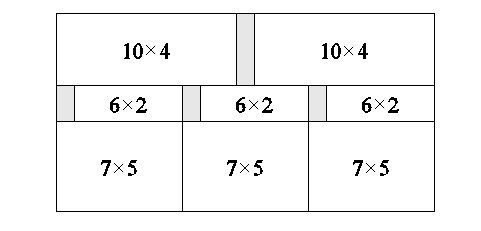
\includegraphics{task2b.jpg}

Напишите программу, которая по размерам изначальной плиты и желаемым размерам
плиток посчитает минимальную суммарную площадь мрамора,
которую придётся выбросить.

